%====================================================================================================
% FaultRecovery: A ampliação da biblioteca de tolerância a falhas
%====================================================================================================
% TCC
%----------------------------------------------------------------------------------------------------
% Autor				: Cleiton Gonçalves de Almeida
% Orientador		: Kleber Kruger
% Instituição 		: UFMS - Universidade Federal do Mato Grosso do Sul
% Departamento		: CPCX - Sistema de Informação
%----------------------------------------------------------------------------------------------------
% Data de criação	: 10 de Maio de 2016
%====================================================================================================

\chapter{Resultados} \label{cap:Resultados}

Neste capítulo são apresentados os resultados dos testes realizados. 

\section{Desempenho da Biblioteca \textit{FaultRecovery}} \label{Sec:tempoRecovery}

Esta seção tem como objetivo demonstrar o quanto a biblioteca \textit{FaultRecovery} pode afetar no tempo de execução de um \textit{firmware}. Para realizar os testes, utilizou-se cinco algoritmos de ordenação \textit{bubble sort, insertion sort, merge sort} e \textit{comb sort} \cite{orderUnicamp, vivaLinux}, a execução dos cinco algoritmos forma um ciclo de teste. Ao todo cada ciclo foi executado cem vezes. Os algoritmos foram implementados para serem executados no microcontrolador \textit{mbed} modelo 1768. Para cada ciclo de teste, utilizou-se um vetor de 4096 elementos, totalizando 4kB de memória. Tentou-se aumentar a quantidade de elementos do vetor, entretanto quando se tentou alocar um espaço de memória maior que 4KB, o \textit{firmware} teve sua execução interrompida no segundo ciclo de teste, em outros no primeiro ciclo.

O primeiro teste tem como objetivo medir o tempo de execução de cada algoritmo de ordenação, simulando um \textit{firmware} implementado por um usuário comum, que não utilização da biblioteca \textit{FaultRecovery}. Todos os algoritmos compartilham do mesmo vetor, por isso, antes de cada ordenação foi necessário desordenar o vetor para cronometrar o tempo real de ordenação. O tempo de cada algoritmo foi cronometrado, desde o início de sua execução até o fim dela, sendo que o tempo de desordenação do vetor foi desprezado.

O segundo teste tem como objetivo medir o tempo de execução dos algoritmos de ordenação, simulando um usuário que utilizou a biblioteca \textit{FaultRecovery}. O tempo de execução no segundo teste foi medido a partir do início da execução de um estado da máquina de estados até o fim dele. Tanto para o primeiro quanto para o segundo teste foi utilizada a mesma quantidade de elementos do vetor (4096), a mesma sequência de execução (\textit{bubble, insertion, selection, merge} \textit{e comb}) e o tempo de desordenação do vetor foi desprezado. Ao final das cem execuções do primeiro e do segundo teste, as médias de tempo de execução para cada algoritmo e para cada ciclo de teste foram calculadas. O tempo de execução da biblioteca \textit{FaultRecovery} também foi calculado, obtendo-se o resultado mostrado na figura \ref{Img:tempoRecovery}.

\begin{figure}[h]
	\centering
	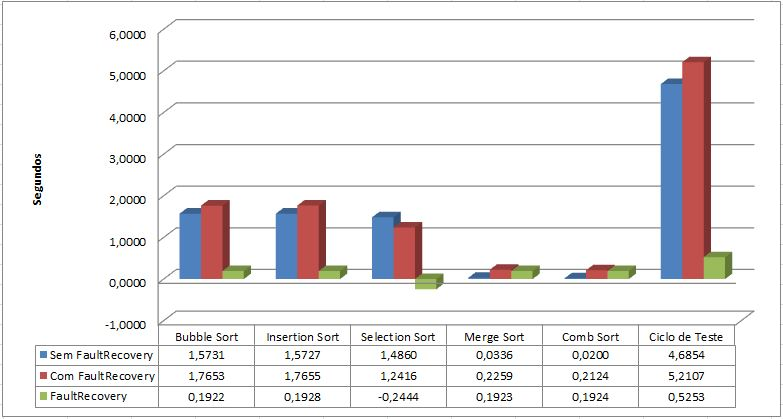
\includegraphics[width=0.9\textwidth]{figuras/tempoRecovery.jpg}
	\caption[Tempo de execução da biblioteca \textit{FaultRecovery}]{Nesta figura são mostrados os resultado dos testes de medição do tempo de execução dos algoritmos de ordenação, sem a biblioteca e com a biblioteca. Percebe-se que com a utilização da biblioteca o tempo de execução dos algoritmos aumentou em média 0,5253 segundos ou 525,3 milisegundos.}
	\label{Img:tempoRecovery}	
	%width=0.5\textwidth (Tamanho da Imagem)
\end{figure}	
\newpage
Dentre os tempos de execução mostrados na figura \ref{Img:tempoRecovery}, obteve-se um resultado inesperado, o esperado seria que o tempo de execução dos algoritmos com a biblioteca \textit{FaultRecovery} fosse maior em relação ao primeiro teste, entretanto o tempo de execução do \textit{insertion sort} foi menor com a biblioteca. Diante disso, verificou-se a implementação dos dois testes, sendo que não foi constatada alguma diferença entre os códigos do primeiro e do segundo teste que pudessem causar este resultado. Após a análise realizou-se um terceiro teste que foi executado cem vezes, utilizou-se um vetor de 3KB, menor que o utilizado nos testes anteriores, para verificar se o comportamento anômalo persistiria. Verificou-se que o comportamento persistiu, sendo que não se disponibiliza de tempo hábil para uma análise e pesquisa aprofundada sobre esse comportamento. Portanto se presume que esses casos são factíveis de ocorrer, provavelmente se deve ao resultado do código gerado pelo compilador, já que o microcontrolador utilizado nos testes não possui sistema operacional e nenhuma outra aplicação rodando simultaneamente. Os resultados do terceiro teste são mostrados na figura \ref{Img:tempoRecovery2}.

\begin{figure}[h]
	\centering
	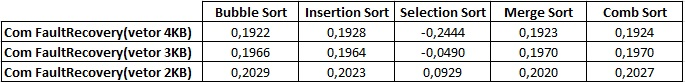
\includegraphics[width=0.9\textwidth]{figuras/tempoRecovery2.jpg}
	\caption[Tempo de execução da biblioteca \textit{FaultRecovery} com três tamanhos de vetores diferentes.]{Nesta figura é mostrado o tempo de execução da biblioteca \textit{FaultRecovery} com três vetores de tamanhos diferentes. Percebe-se que o tempo de execução da biblioteca no algoritmo \textit{insertion sort} é negativo no primeiro e segundo teste, contudo no teste com o vetor de tamanho 2KB, obteve-se um tempo de execução positivo. Portanto, pode-se concluir que quando a quantidade dados a serem processadas for grande, provavelmente o compilador optimiza o código compilado.}
	\label{Img:tempoRecovery2}	
	%width=0.5\textwidth (Tamanho da Imagem)
\end{figure}
\newpage
\section{Desempenho e Eficiência da Classe TData} \label{Sec:tempoTData}

Para testar a redundância de dados da classe TData e se a sua utilização pode causar alguma perda de desempenho em algum \textit{firmware}, foram realizados dois tipos de testes. O primeiro não utilizando a classe TData e o segundo utilizando-a, em ambos os testes foram realizados cem ciclos de execução, conforme descrito no primeiro parágrafo da seção \ref{Sec:tempoRecovery}. No entanto houve a necessidade de reduzir o tamanho do vetor de 4096 para 1024 elementos, devido a redundância de dados da classe TData, pois ela copia um valor para três endereços de memória diferentes. Se fossem utilizados os 4096 elementos a quantidade de memória alocada seria de aproximadamente 16KB, impossibilitando a realização dos testes. O teste que não utilizada a classe TData tem como objetivo medir o tempo de execução de cada algoritmo de ordenação, sendo que a biblioteca \textit{FaultRecovery} não foi utilizada, foram levados em conta apenas o tempo de execução de cada algoritmo. O resultado do primeiro teste foi comparado com o do segundo, obtendo-se o tempo de execução da classe TData conforme demonstrado na figura \ref{Img:tempoTData}. Para iniciar o segundo teste, epenas foi necessário substituir a declaração do vetor de \textit{unsigned short vetor[n]} para um \textit{TData$<$unsigned short$>$ vetor[n]}, com isso a redundância de dados disponível na classe TData pode ser aplicada nos dados do vetor.

Notou-se uma diferença média 0,2658 segundos do tempo de execução de um algoritmo de ordenação sem redundância de dados para um com redundância de dados. No entanto, deve-se levar em conta que o teste realizado sem a classe TData estava sujeito a falhar em algum ciclo de teste e foi o que aconteceu, na figura \ref{Img:falhaTData} têm-se o resultado da execução do primeiro e do segundo teste. Foram determinados três parâmetros de teste para determinar se um ciclo de teste falhou ou não. Como o vetor possui 1024 elementos e o resultado de uma ordenação que inicia em 1 até 1024 é conhecida, após a injeção de falhas no microcontrolador \textit{mbed}, alterando um endereço de memória aleatório, estabeleceu-se que para um ciclo de teste falhar ele deve ter 10\%, 25\% ou 50\% dos 1024 elementos diferentes do resultado conhecido. 

Para os resultados acima de 10\%, 25\% e 50\% analisou-se os algoritmos de ordenação isoladamente e também cada ciclo de teste, lembrando que cada ciclo é representado pela execução dos cinco algoritmos de ordenação. Obteve-se os seguintes resultados, para os valores acima de 10\%, 25\% e 50\% de falhas respectivamente, 44\%, 25\% e 20\% dos ciclos de testes falharam. Percebe-se que o primeiro teste não possui redundância de dados, embora os cem ciclos de testes tenham sido executados, pode-se notar que os valores do vetor não continuaram os mesmos após a injeção de falhas. No entanto na figura \ref{Img:falhaTData} é possível visualizar que mesmo após as injeções de falhas, a classe TData se mostrou eficaz garantindo a consistência dos dados do vetor até o fim dos cem ciclos de teste.


\begin{figure}[h]
	\centering
	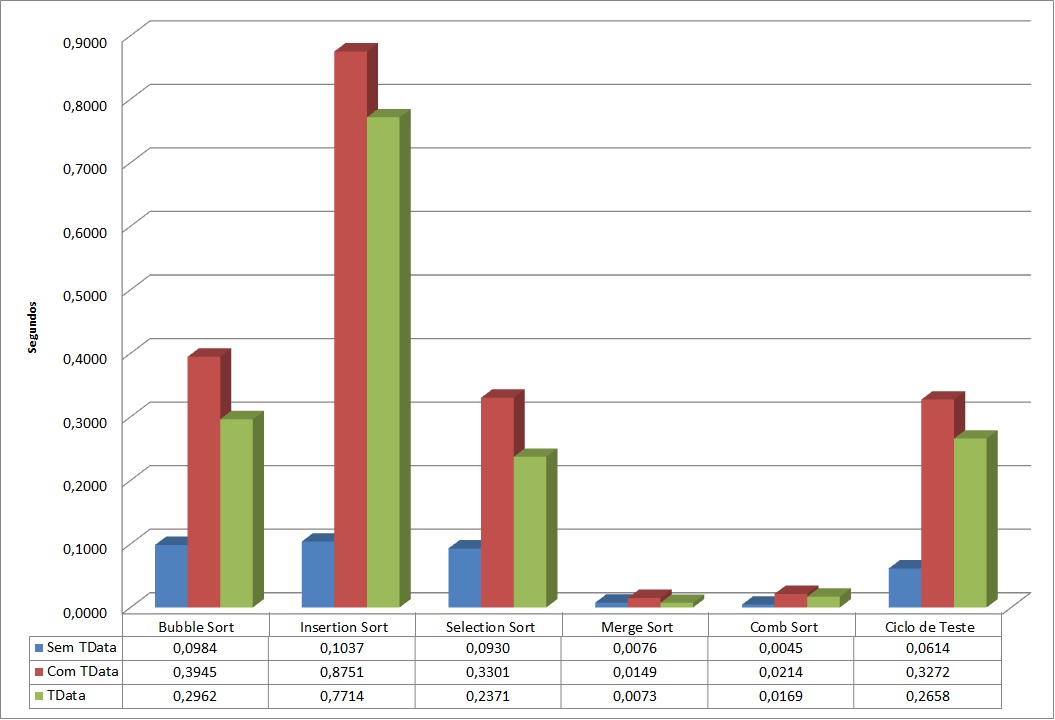
\includegraphics[width=0.9\textwidth]{figuras/tempoTData.jpg}
	\caption[Tempo de execução da Classe TData ]{O tempo de execução dos algoritmos sem a classe TData foi relativamente baixo, sendo que o maior tempo atingiu 0,1037 segundos ou 103,7 milisegundos para ordenar um vetor de 1024 elementos. Já o tempo dos algoritmos com a Classe TData foi um pouco maior, sendo o tempo de execução do algoritmo \textit{insertion sort} que atingiu 0,8751 segundos ou 875,1 milisegundos. O tempo de execução médio da classe TData para cada algoritmo de ordenação foi de 0,2658 segundos ou 265,8 milisegundos.}
	\label{Img:tempoTData}	
	%width=0.5\textwidth (Tamanho da Imagem)
\end{figure}

\begin{figure}[h]
	\centering
	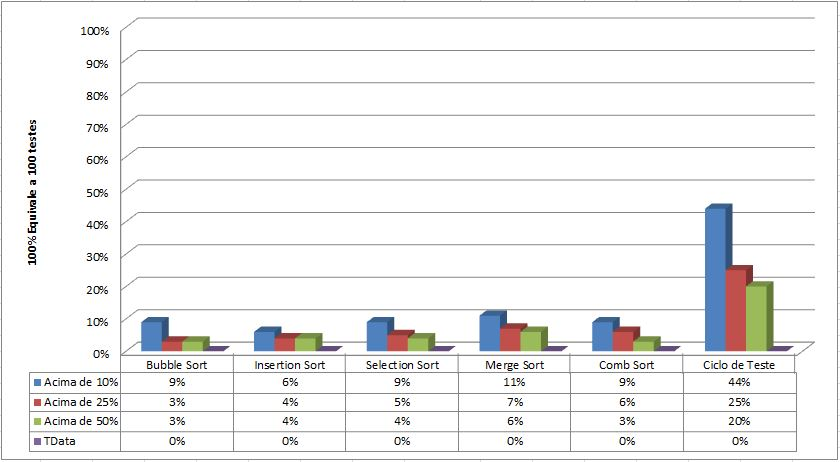
\includegraphics[width=0.9\textwidth]{figuras/falhaTData.jpg}
	\caption[Teste de redundância de dados da classe TData ]{Nesta figura para as falhas detectadas acima de 10\%, 25\% e 50\% são do teste que não utiliza redundância de dados, por exemplo, para as falhas acima de 10\%, aproximadamento 44\% dos ciclos de testes falharam. No entanto para o teste que utilizou a redundância de dados disponibilizada pela TData nenhum algoritmo de ordenação e ciclo de teste falharam, ou seja, embora o teste estivesse sendo bombardeado por falhas, a classe TData se mostrou eficaz corrigindo os valores alterados nos endereços de meória cobertos pela redundância de dados.}
	\label{Img:falhaTData}	
	%width=0.5\textwidth (Tamanho da Imagem)
\end{figure}

\newpage
\section{Recuperação de falhas da biblioteca \textit{FaultRecovery}}\label{Sec:recupeFault}

Esta seção mostra os resultados dos teste realizados com a biblioteca \textit{FaultRecovery}. O código utilizado na seção \ref{Sec:tempoRecovery} foi modificado para injetar falhas em endereços de memória aleatórios. Foram utilizados os mesmos algoritmos de ordenação, no entanto o tempo de execução da biblioteca foi desprezado, pois o resultado avaliado neste teste foi a capacidade de recuperação de falhas. Se as falhas registradas nos resultados ocorressem em uma situação real, os dados afetados por essas falhas poderiam ocasionar o travamento do \textit{firmware}. Neste caso, quando o \textit{whatchdog} percebesse que o microcontrolador estivesse travado, o \textit{mbed} seria reinicializado. No entanto se o travamento ocorresse no momento em que os dados coletados por uma estação meteorológica fossem enviados para um servidor remoto, por ser uma máquina de estados, no qual a ordem de execução de cada estado implica nos resultados obtidos, quando o \textit{mbed} fosse reinicializado, o primeiro estado que seria executado, poderia ou não ser o estado responsável que enviaria os dados ao servidor remoto. 

Para que isso não venha a ocorrer, a estação meteorológica poderia ser implementada utilizando a biblioteca \textit{FaultRecovery} para que pontos de recuperação de falhas pudessem ser criados, para assim que o microcontrolador reinicializa-se por conta de alguma falha, algum ponto de recuperação predefinido pudesse ser executado. Porém neste trabalho não se implementou uma estação meteorológica para simular esse acontecimento. Entretanto utilizou-se algoritmos de ordenação para simular uma máquina de estados. Foram criados pontos de recuperação para cada algoritmo de ordenação, se em algum momento o microcontrolador vier a travar e posteriormente ser reiniciado, seja manualmente ou automaticamente, o ponto de recuperação predefinido será executado. Mostra-se na figura \ref{Img:testeFaultRecovery} os resultados obtidos após a execução de cem ciclos de testes, cada ciclo é representado pela execução dos cinco algoritmos de ordenação conforme descrito na seção \ref{Sec:tempoRecovery}. 


\begin{figure}[h]
	\centering
	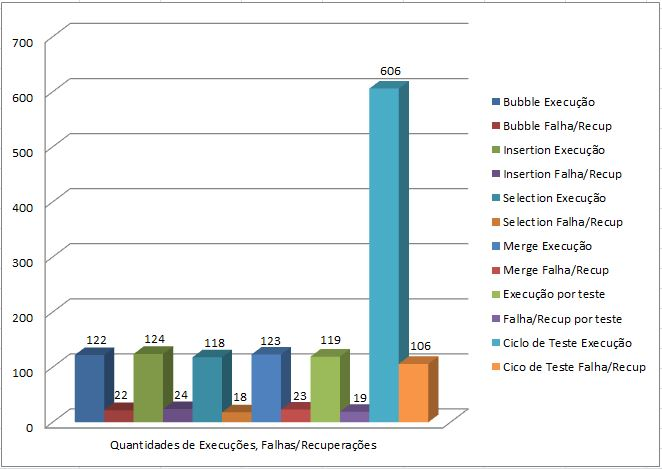
\includegraphics[width=0.9\textwidth]{figuras/testeFaultRecovery.jpg}
	\caption[Resultados Obtidos da Biblioteca \textit{FaultRecovery}]{Esta figura mostra a quantidade de execuções e falhas de cada algoritmo, inclusive de cada ciclo de teste. Por exemplo, a primeira coluna, da esquerda para e direita, representa o número de execuções do algoritmo \textit{bubble sort}, pode-se perceber que embora tenham sido executados cem ciclos de teste, o algoritmo foi executado cento e vinte e duas vezes. Em contra partida, na segunda coluna, que representa a quantidade de vezes em que um ponto de recuperação do \textit{bubble sort} foi executado, o \textit{firmware} reinicializou, e executou o ponto de recuperação do \textit{bubble sort} vinte e duas vezes.}
	\label{Img:testeFaultRecovery}	
	%width=0.5\textwidth (Tamanho da Imagem)
\end{figure}


\section{Injeção de Falhas com a Biblioteca \textit{FaultInjector}}

Esta seção mostra o resultado de injeção de falhas na memória flash do microcontrolador \textit{mbed} modelo 1768. A injeção de falhas na memória flash sorteia um setor aleatório para injetar uma quantidade predefinida de falhas, que podem variar de 256, 512, 1024 ou 4096 bytes. Na figura \ref{Img:injecaoFlash} é exibido um teste em que foram injetadas 256 bytes de falhas no setor 25, que foi sorteado aleatoriamente pelo injetor de falhas. O endereço de memória do setor sorteado em hexadecimal inicia em 0x00058000 e termina em 0x0005FFFF. Pode-se perceber que os bytes dos endereços de memória do setor 25 (0x00058000 até 0x000580F0) foram alterados. Portanto agora a biblioteca \textit{FaultInjector} pode injetar falhas na memória flash do microcontrolador \textit{mbed} modelo 1768.

\begin{figure}
	\centering
	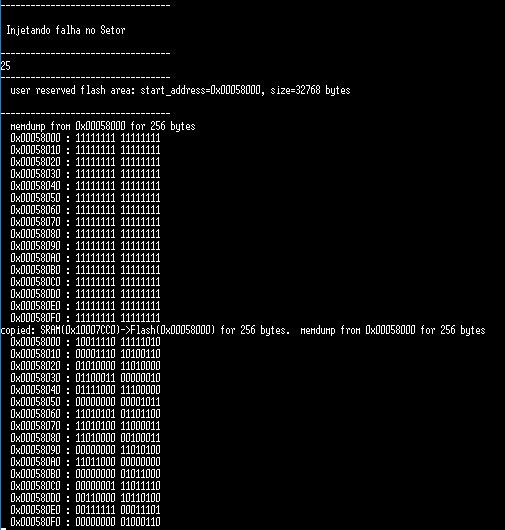
\includegraphics[width=0.9\textwidth]{figuras/injecaoFlash.jpg}
	\caption[Injeção de Falhas na Memória Flash]{Nesta figura é mostrado o setor da memória flash soteado pelo injetor de falhas e os endereços desse setor. Além de mostrar como os bits se encontravam antes de serem modificados, assim como também pode ser visualizada a modificação desses bits. }
	\label{Img:injecaoFlash}	
	%width=0.5\textwidth (Tamanho da Imagem)
\end{figure}